\documentclass[11pt]{article}
\usepackage[letterpaper,margin=0.68in,headheight=15pt]{geometry}
\usepackage[T1]{fontenc}
\usepackage{lmodern}
\usepackage{amsmath,amssymb}
\usepackage{array,booktabs,enumitem,multicol}
\usepackage{xcolor}
\usepackage{tikz}
\usepackage{fancyhdr}
\usepackage{microtype}
\setlength{\parindent}{0pt}
\setlength{\parskip}{5pt}
\definecolor{olive}{HTML}{555B35}
\definecolor{gold}{HTML}{B18A22}
\definecolor{soft}{HTML}{F4F1DE}
\definecolor{bluegray}{HTML}{E8EEF2}
\pagestyle{fancy}
\fancyhf{}
\fancyhead[L]{\textcolor{olive}{\small MATH\& 141: Precalculus I}}
\fancyhead[R]{\textcolor{gold}{\small Fall 2026}}
\fancyfoot[C]{\thepage}
\renewcommand{\headrulewidth}{0.45pt}
\renewcommand{\footrulewidth}{0pt}
\setlist[enumerate]{leftmargin=*,itemsep=0.08in,topsep=0.05in}
\newcommand{\assessmenttitle}[2]{%
  {\Large\bfseries Module #1: #2}\par\vspace{3pt}
}
\newcommand{\studentline}{%
\noindent\textbf{Name:}\hspace{2.6in}\textbf{Date:}\hspace{1.15in}\par\vspace{7pt}}
\newcommand{\directions}[1]{\textit{#1}\par\vspace{4pt}}
\newcommand{\answerblank}[1]{\vspace{#1}}
\newcommand{\blankgrid}[4]{%
\begin{center}
\begin{tikzpicture}[x=0.75cm,y=0.75cm]
  \draw[step=1,gray!28,very thin] (#1,#3) grid (#2,#4);
  \draw[->,thick] (#1,0)--(#2,0) node[right] {$x$};
  \draw[->,thick] (0,#3)--(0,#4) node[above] {$y$};
  \foreach \x in {#1,...,#2}{\ifnum\x=0\else\draw (\x,0.10)--(\x,-0.10) node[below=2pt,font=\scriptsize]{\x};\fi}
  \foreach \y in {#3,...,#4}{\ifnum\y=0\else\draw (0.10,\y)--(-0.10,\y) node[left=2pt,font=\scriptsize]{\y};\fi}
\end{tikzpicture}
\end{center}}
\newcommand{\smallgrid}[4]{%
\begin{tikzpicture}[x=0.50cm,y=0.50cm]
  \draw[step=1,gray!28,very thin] (#1,#3) grid (#2,#4);
  \draw[->,thick] (#1,0)--(#2,0) node[right] {$x$};
  \draw[->,thick] (0,#3)--(0,#4) node[above] {$y$};
\end{tikzpicture}}
\begin{document}

% MODULE 1 PREQUIZ
\assessmenttitle{1}{Functions -- Prequiz}
\studentline
\directions{Four short questions. Show enough work that you can find the step where an error occurred.}
\begin{enumerate}
\item Consider the relation
\[
R=\{(-2,5),(0,1),(3,4),(0,-2)\}.
\]
Does this relation define a function? Explain briefly.
\answerblank{0.48in}

\item Let $f(x)=2x^2-3x+1$. Find $f(-2)$.
\answerblank{0.55in}

\item The graph of $y=f(x)$ is transformed to
\[
g(x)=f(x-3)-2.
\]
Describe the horizontal and vertical shifts in words.
\answerblank{0.52in}

\item The point $(1,4)$ lies on the graph of $y=f(x)$. Where does this point move on the graph of
\[
y=-2f(x+1)+3?
\]
\answerblank{0.62in}
\end{enumerate}
\newpage

% MODULE 1 CHECKIN PAGE 1
\assessmenttitle{1}{Functions -- Weekly Check-In}
\studentline
\directions{Three questions. Show enough work to make your reasoning clear.}
\textbf{1. Relations and functions.}

Consider the relation
\[
R=\{(-4,1),(-1,3),(2,5),(4,3),(-1,-2)\}.
\]
Does this relation define a function? State \emph{yes} or \emph{no} and explain using the input-output definition of a function.
\answerblank{1.10in}

\textbf{2. Function values and transformed points.}

Let $f(x)=2x^2-3x+1$.
\begin{enumerate}[label=(\alph*),leftmargin=0.35in]
\item Find $f(-2)$.
\answerblank{0.42in}
\item Suppose the point $(1,4)$ lies on the graph of $y=h(x)$. Where does that point move on the graph of
\[
y=-2h(x+1)+3?
\]
Show how the coordinates change.
\answerblank{0.58in}
\end{enumerate}
\newpage

% MODULE 1 CHECKIN PAGE 2
\assessmenttitle{1}{Functions -- Weekly Check-In, continued}
\studentline
\textbf{3. Transforming an unknown graph.}

The graph of $y=f(x)$ is shown below. On the \emph{same coordinate plane}, graph
\[
y=-f(x-2)+1.
\]
Show the transformed locations of all five marked points and connect them with the same shape as the original graph.

\begin{center}
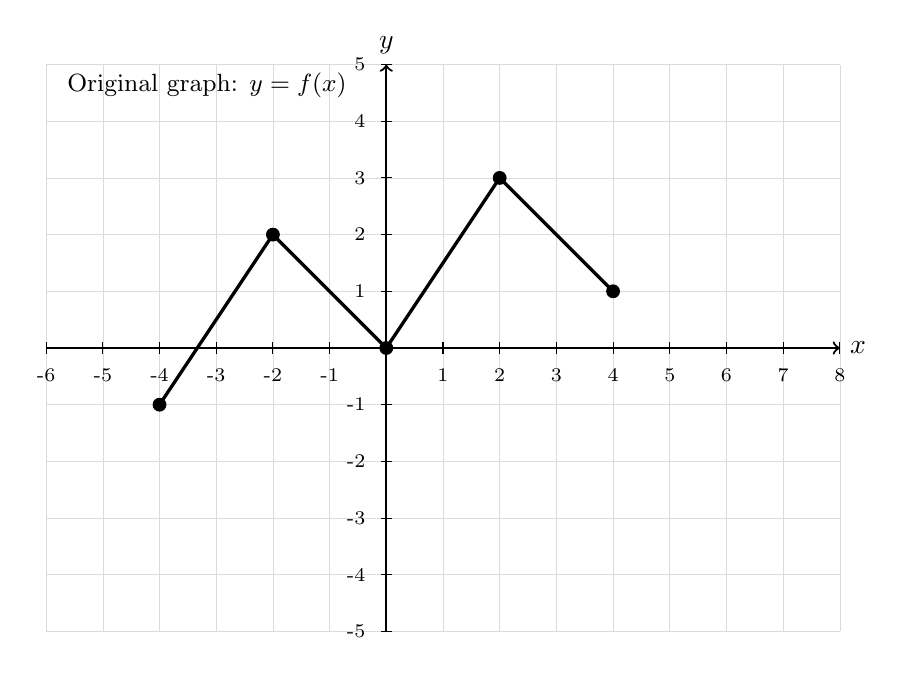
\begin{tikzpicture}[x=0.72cm,y=0.72cm]
  \draw[step=1,gray!28,very thin] (-6,-5) grid (8,5);
  \draw[->,thick] (-6,0)--(8,0) node[right] {$x$};
  \draw[->,thick] (0,-5)--(0,5) node[above] {$y$};
  \foreach \x in {-6,...,8}{\ifnum\x=0\else\draw (\x,.1)--(\x,-.1) node[below=2pt,font=\scriptsize]{\x};\fi}
  \foreach \y in {-5,...,5}{\ifnum\y=0\else\draw (.1,\y)--(-.1,\y) node[left=2pt,font=\scriptsize]{\y};\fi}
  \draw[very thick] plot coordinates {(-4,-1) (-2,2) (0,0) (2,3) (4,1)};
  \foreach \p in {(-4,-1),(-2,2),(0,0),(2,3),(4,1)} \fill \p circle (2.5pt);
  \node[anchor=south west,font=\small] at (-5.8,4.25) {Original graph: $y=f(x)$};
\end{tikzpicture}
\end{center}

\textit{Below the graph, list the five transformed points as ordered pairs.}
\answerblank{0.55in}

\end{document}
